\documentclass[a4paper,12pt,times,numbered,print,index]{Classes/PhDThesisPSnPDF}
\usepackage{qtree}
\ifsetCustomMargin
  \RequirePackage[left=37mm,right=30mm,top=35mm,bottom=30mm]{geometry}
  \setFancyHdr
\fi

\ifsetCustomFont
  \RequirePackage{helvet}
\fi

\RequirePackage[labelsep=space,tableposition=top]{caption}
\renewcommand{\figurename}{Fig.}

\usepackage{subcaption}


\usepackage{booktabs}
\usepackage{multirow}

\usepackage{amsfonts}
\usepackage{amsmath}
\usepackage{amssymb}
\usepackage{siunitx}

\ifuseCustomBib
   \RequirePackage[square, sort, numbers, authoryear]{natbib}

\fi

\renewcommand{\bibname}{References}

\setcounter{secnumdepth}{2}
\setcounter{tocdepth}{2}



\title{The LEXenstein Manual}

\author{Gustavo Henrique Paetzold}

\crest{
\includegraphics[width=0.50\textwidth]{Figs/frankenstein_monster.png}}

\usepackage{listings}
\usepackage{color}
\usepackage{amsmath}

\definecolor{dkgreen}{rgb}{0,0.6,0}
\definecolor{gray}{rgb}{0.5,0.5,0.5}
\definecolor{mauve}{rgb}{0.58,0,0.82}

\lstset{frame=tb,
  language=Python,
  aboveskip=3mm,
  belowskip=3mm,
  showstringspaces=false,
  columns=flexible,
  basicstyle={\small\ttfamily},
  numbers=none,
  numberstyle=\tiny\color{gray},
  keywordstyle=\color{blue},
  commentstyle=\color{dkgreen},
  stringstyle=\color{mauve},
  breaklines=true,
  breakatwhitespace=true,
  tabsize=3
}

\begin{document}

\frontmatter

\begin{titlepage}
  \maketitle
\end{titlepage}

\tableofcontents

\mainmatter

\chapter{Introduction}

LEXenstein is a framework for Lexical Simplification. It contains several methods, tools and resources for one to easily create Lexical Simplification systems and test them in various distinct ways. It takes Lexical Simplification as a process that can be modeled as a pipeline of sub-processes, as illustrated in Figure~\ref{fig:exlepipe}.

\begin{figure}[htbp!] 
\centering    
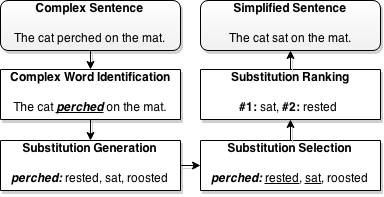
\includegraphics[scale=0.8]{Figs/diagramshadow.png}
\caption{Lexical Simplification pipeline}
\label{fig:exlepipe}
\end{figure}

Each task in Figure~\ref{fig:exlepipe} can be described as:

\begin{enumerate}
\item \textbf{Complex Word Identification}: Task of deciding which words of a given sentence may not be understood by a given target audience and hence must be simplified.

\item \textbf{Substitution Generation}: Task of finding pairs of words or expressions that share the same meaning and are interchangeable in some context.

\item \textbf{Substitution Selection}: Task of deciding which is the meaning of a given complex ambiguous word in a sentence to be simplified, and then selecting which substitutions available also represent that meaning.

\item \textbf{Substitution Ranking}: Task of ranking the remaining substitutions of a given complex word by their simplicity.
\end{enumerate}

Its name is a reference to the \textit{Frankenstein} novel, published by \cite{frankenstein}. It refers to the fact that one can, as Victor Frankenstein did, create an entire Lexical Simplification ``creature'' by combining multiple ``pieces'' of the Lexical Simplification pipeline together.

LEXenstein is divided in several modules: Complex Word Identification, Substitution Generation, Substitution Selection, Substitution Ranking, Feature Estimation, Evaluation, Text Adorning, Spelling Correction and Utilities. In the next Sections, we describe the VICTOR and CWICTOR file formats, explain how to properly setup LEXenstein, and discuss in detail the components included in each module of the framework.
\chapter{Installation}
\label{install}

LEXenstein is a library written entirely in Python. It hence requires for Python $2$.$7$.* to be installed in the user's machine. We have not yet tried to run LEXenstein over Python $3$.*. To install LEXenstein, please follow the steps below:

\begin{enumerate}
	\item Download and unpack the tool from \url{http://ghpaetzold.github.io/LEXenstein/}.
	\item Navigate to the tool's root folder.
	\item Run the following command line:
	
	\begin{lstlisting}
	python setup.py install
	\end{lstlisting}
	
	\item If you don't with to install the tool in your Python distribution, you can alternatively copy the ``lexenstein'' folder into the folder of your project.
	\item Access LEXenstein by importing its modules in the following fashion:
	\begin{lstlisting}
from lexenstein.morphadorner import *
from lexenstein.spelling import *
from lexenstein.features import *
from lexenstein.identifiers import *
from lexenstein.generators import *
from lexenstein.selectors import *
from lexenstein.rankers import *
from lexenstein.evaluators import *
from lexenstein.util import *
\end{lstlisting}
\end{enumerate}

LEXenstein requires for several libraries and toolkits to be included in the user's Python $2$.$7$.* installation. The following Sections explain which libraries and toolkits are required, where to get them and how to install them.






\section{Required Tools and Libraries}

\subsection{Morph Adorner Toolkit}

The Morph Adorner Toolkit \cite{Paetzold15mat} is a set of Java applications that facilitate the access to Morph Adorner's functionalities \cite{morphadorner}. This tool is used by LEXenstein's Substitution Generation module to create inflections for generated substitutions. To install it, follow the steps below:

\begin{enumerate}
	\item Download the tool from \url{http://ghpaetzold.github.io/MorphAdornerToolkit/}
	\item Place it in a folder of your choice
\end{enumerate}

Since the tool does not require any compilation, all you need to do is use the path in which you installed it to create instances of the \textbf{MorphAdornerToolkit} class, which can be found in LEXenstein's Morph Adorning module.








\subsection{NLTK}

NLTK \cite{nltk} is a set of resources and algorithms for tasks related, but not restricted to, Natural Language Processing. To install it, please follow the steps provided in: \url{http://www.nltk.org/install.html}. Once you have NLTK installed in your Python distribution, please download all additional resources available by following this tutorial: \url{http://www.nltk.org/data.html}.






\subsection{KenLM}

KenLM \cite{kenlm} is a tool for fast language model creation and querying. LEXenstein's modules use KenLM to access the data in binary language models for various tasks, such as feature calculation and substitution filtering. To install it, please follow the steps below:

\begin{enumerate}
	\item Download or clone KenLM from \url{https://github.com/kpu/kenlm}
	\item Place it in a folder of your choice
	\item Navigate to the installation folder in a terminal and run: \textbf{python setup.py install}
\end{enumerate}

If no problems occur, KenLM should now be installed in your Python distribution. To verify whether or not the installation was successful, open Python and try importing the library with the following line of code: \textbf{import kenlm}. If no errors occur, then the installation was successful.







\subsection{Scipy and Numpy}

Scipy and Numpy \cite{scipy} are tools that offer great utility for projects and applications in the fields of mathematics, science, and engineering. To install them, please follow the instructions in: \url{http://www.scipy.org/install.html}.







\subsection{Gensim}

Gensim \cite{gensim} is a set of algorithms for unsupervised semantic modeling. LEXenstein uses Gensim to read word vector models. To install it, follow the instructions in: \url{https://radimrehurek.com/gensim/install.html}.







\subsection{PyWSD}

PyWSD \cite{pywsd} is a library that offers access to several Word Sense Disambiguation algorithms. LEXenstein's uses this library to filter substitutions. To install it, follow the steps below:

\begin{enumerate}
	\item Download or clone PyWSD from \url{https://github.com/alvations/pywsd}
	\item Place it in a folder of your choice
	\item Navigate to the installation folder in a terminal and run: \textbf{python setup.py install}
\end{enumerate}

If no problems occur, PyWSD should now be installed in your Python distribution. To verify whether or not the installation was successful, open Python and try importing the library with the following line of code: \textbf{import pywsd}. If no errors occur, then the installation was successful.






\subsection{Scikit-Learn}

Scikit-Learn \cite{scikit-learn} is a set of tools for data mining, data analysis and machine learning. LEXenstein uses this library to learn ranking models. To install it, follow the instructions in: \url{http://scikit-learn.org/stable/install.html}.



\subsection{SVM-Rank}

SVM-Rank \cite{svmrank} is a tool that allows for one to use Support Vector Machines in ranking setups. LEXenstein uses this library to learn ranking models. To install it, follow the instructions in: \url{http://www.cs.cornell.edu/people/tj/svm_light/svm_rank.html}.


\subsection{Stanford Tagger}

The Stanford Tagger \cite{stanfordparser} is a tool that allows for one to annotate sentences with Part-of-Speech (POS) tags. LEXenstein uses this library to find the POS tag of a target word in a sentence. To install it, download the application's latest version from \url{http://nlp.stanford.edu/software/tagger.shtml}. Inside the package, you will be able to find the \textbf{stanford-tagger.jar} executable and pre-trained tagging models inside the \textbf{/models/} folder required by some of LEXenstein's substitution generators.



\subsection{Other Libraries}

LEXenstein also uses various other well-known Python modules, they are: xml, re, urllib$2$, subprocess, codecs and os.
\chapter{Resources}
\label{chapterresources}

Throughout the following Chapters, you will find usage examples of all classes and functions in LEXenstein. These examples will refer to various sample resources, such as:

\begin{itemize}
	\item \textbf{corpus.txt}: A corpus of text. We recommend for the corpus to be tokenized and truecased.
	
	\item \textbf{spelling\_model.bin}: A binary spelling model trained with the NorvigCorrector class from the Spelling Correction module.
	
	\item \textbf{morph}: The Morph Adorner Toolkit \cite{Paetzold15mat}.
	
	\item \textbf{lexicon.txt}: A vocabulary. It must contain one word per line.
	
	\item \textbf{embeddings\_model.bin}: A binary word embeddings model trained with word2vec \cite{mikolov2013efficient}. For more information on how to create them, please follow the instructions on the website of the application at \url{https://code.google.com/p/word2vec/}.
	
	\item \textbf{tagged\_embeddings\_model.bin}: A binary word embedding models trained with word2vec \cite{mikolov2013efficient} over a corpus annotated with generalized POS tags following the convention used by the ``getGeneralisedPOS'' function from the Utilities model.
	
	To create your own tagged word vector model, you must:
	
		\begin{enumerate}
			\item Produce POS tags for a large corpus of text.
			\item Concatenate the POS tags to each word in the corpus using the format of Example~\ref{eq:taggedw2v}, where $w_{i}$ is the $i$th word in a sentence, and $p_{i}$ its POS tag.
			
			\begin{equation}
				\label{eq:taggedw2v}
				w_{1}|||p_{1}\; w_{2}|||p_{2}\;  ...\; w_{n-1}|||p_{n-1}\; w_{n}|||p_{n}
				\end{equation}
				
			\item Train a binary word vector model over the resulting corpus using word$2$vec.
		\end{enumerate}
		
		LEXenstein supports two POS tag conventions:
		
			\begin{enumerate}
				\item Treebank: POS tags in the Penn Treebank format \cite{Marcus1993}. They can be produced by any modern POS tagger, such as the Stanford Tagger \cite{stanfordparser}.
				
				\item Paetzold: Generalized versions of Treebank tags. They can be derived from Treebank tags using the ``getGeneralisedPOS'' from the LEXenstein's Utilities module (lexenstein.util).
			\end{enumerate}
	
	\item \textbf{lm.bin}: A binary language model trained with KenLM \cite{kenlm}. Language models used by LEXenstein can be produced with the following command lines:

			\begin{lstlisting}
			lmplz -o [order] <[corpus_of_text] >[language_model]
			\end{lstlisting}
			\begin{lstlisting}
			build_binary [language_model] [binary_language_model]
			\end{lstlisting}
			
		The user can also use other language modeling tools, such as SRILM, to produce a language model in ARPA format, and then binarize it with KenLM.
		
	
	\item \textbf{lm\_complex.bin}: A binary language model trained with KenLM \cite{kenlm} over texts of complex nature.
	
	\item \textbf{lm\_simple.bin}: A binary language model trained with KenLM \cite{kenlm} over texts of simple nature.
	
	
	\item \textbf{translation\_probs.bin}: A binary translation probabilities file produced with the ``addTranslationProbabilitiesFileToShelve'' function from the Utilities module.
	
	\item \textbf{cond\_prob.bin}: A binary POS tag conditional probability model trained with the ``createConditionalProbabilityModel'' function from the Utilities module.
	
	\item \textbf{pos\_model.tagger}: A POS tagging model in the format used by the Stanford Tagger \cite{stanfordparser}. You can find Stanford Tagger models in the tool's webpage\footnote{http://nlp.stanford.edu/software/tagger.shtml}, inside the ``models'' folder. They will have a ``.tagger'' extension.
	
	\item \textbf{stanford-postagger.jar}: The Stanford Tagger \cite{stanfordparser}. You can find the Stanford Tagger in the tool's webpage\footnote{http://nlp.stanford.edu/software/tagger.shtml}.
	
	\item \textbf{lexmturk.txt}: A sample of the LexMTurk dataset \cite{Horn2014} in VICTOR format.
	
	\item \textbf{train\_cwictor\_corpus.txt}: A sample of the training set from the Complex Word Identification task of SemEval 2016 \cite{Paetzold2016SemEval} in CWICTOR format.
	
	\item \textbf{test\_cwictor\_corpus.txt}:  A sample of the test set from the Complex Word Identification task of SemEval 2016 \cite{Paetzold2016SemEval} in CWICTOR format.
	
	\item \textbf{parallel.txt}: A file containing complex-to-simple POS tagged aligned sentences. Each line of the parsed parallel document must be in the format described in Example~\ref{parsedparallel}, where $w_{i}^{s}$ is a word in position $i$ of a source sentence $s$, $p_{i}^{s}$ its POS tag, $w_{j}^{t}$ is a word in position $j$ of a target sentence $t$, and $p_{j}^{t}$ its POS tag.

\begin{equation}
\label{parsedparallel}
\left \langle w_{0}^{s} \right \rangle\! |||\! \left \langle p_{0}^{s} \right \rangle\cdots\left \langle w_{n}^{s} \right \rangle\!|||\!\left \langle p_{n}^{s} \right \rangle \;\; \left \langle w_{0}^{t} \right \rangle\! |||\! \left \langle p_{0}^{t} \right \rangle\cdots\left \langle w_{n}^{t} \right \rangle\!|||\!\left \langle p_{n}^{t} \right \rangle
\end{equation}

All tokens of form $\left \langle w_{i}^{s} \right \rangle\! |||\! \left \langle p_{i}^{s} \right \rangle$ are separated by a blank space, and the two set of source and target tokens $\left \langle w_{0}^{s} \right \rangle\! |||\! \left \langle p_{0}^{s} \right \rangle\cdots\left \langle w_{n}^{s} \right \rangle\!|||\!\left \langle p_{n}^{s} \right \rangle$ are separated by a tabulation marker.
	
	\item \textbf{alignments.txt}: A file containing word alignments between the sentences in ``parallel.txt''. The alignments must be in Pharaoh format, and can be produced easily with the help of fast-align\footnote{https://github.com/clab/fast\_align}. Each line of the alignments file must be structured as illustrated in Example~\ref{pharaoh}, where $\left \langle i_{h}^{s} \right \rangle$ is an index $i$ in source sentence $s$, and $\left \langle j_{h}^{t} \right \rangle$ is the index $j$ in source sentence $t$ aligned to it.

\begin{equation}
\label{pharaoh}
\left \langle i_{0}^{s} \right \rangle\! -\! \left \langle j_{0}^{t} \right \rangle\; \left \langle i_{1}^{s} \right \rangle\! -\! \left \langle j_{1}^{t} \right \rangle\cdots\left \langle i_{n-1}^{s} \right \rangle\! -\! \left \langle j_{n-1}^{t} \right \rangle\; \left \langle i_{n}^{s} \right \rangle\! -\! \left \langle j_{n}^{t} \right \rangle
\end{equation}

All tokens of form $\left \langle i_{h}^{s} \right \rangle\! -\! \left \langle j_{h}^{t} \right \rangle$ are separated by a blank space.
	
	\item \textbf{stop\_words.txt}: A list of stop words. Each line must contain a single word.
	
	\item \textbf{vocab\_complex.txt}: A vocabulary extracted from texts of complex nature. Each line must contain a single word.
	
	\item \textbf{vocab\_simple.txt}: A vocabulary extracted from texts of simple nature. Each line must contain a single word.
	
	\item \textbf{cooc\_model.txt}: A word co-occurrence model. The model must be in plain text format, and each line must follow the format illustrated in Example~\ref{cooc}, where $\left\langle w_{i} \right\rangle$ is a word, $\left\langle c_{i}^{j} \right\rangle$ a co-occurring word and $\left\langle f_{i}^{j} \right\rangle$ its frequency of appearance.

\begin{equation}
\label{cooc}
\left\langle w_{i} \right\rangle\; \left\langle c_{i}^{0} \right\rangle\!:\!\left\langle f_{i}^{0} \right\rangle\;\left\langle c_{i}^{1} \right\rangle\!:\!\left\langle f_{i}^{1} \right\rangle\cdots\left\langle c_{i}^{n-1} \right\rangle\!:\!\left\langle f_{i}^{n-1} \right\rangle \; \left\langle c_{i}^{n} \right\rangle\!:\!\left\langle f_{i}^{n} \right\rangle
\end{equation}

Each component in the format above must be separated by a tabulation marker. To create a co-occurrence model, either create a script that does so, or use the ``produceWordCooccurrenceModel'' function from the utilities module (lexenstein.util).
	
	\item \textbf{clusters.txt}: A list of word clusters. The file must be in plain text format, and each line must follow the format illustrated in Example~\ref{clusterfile}, which is the one adopted by the Brown Clusters implementation of \cite{brownclusters}. In the Example~\ref{clusterfile}, $c_{i}$ is a class identifier, $w_{i}$ a word, and $f_{i}$ an optional frequency of occurrence of word $w_{i}$ in the corpus over which the word classes were estimated.

\begin{equation}
\label{clusterfile}
\left\langle c_{i} \right\rangle\; \left\langle w_{i} \right\rangle \left\langle f_{i} \right\rangle
\end{equation}

Each component in the format above must be separated by a tabulation marker. To create the file, one can use the software provided at \url{https://github.com/percyliang/brown-cluster}. Once the tool is installed, run the following command line:

\begin{lstlisting}
./wcluster --text <corpus_of_sentences> --c <number_of_clusters>
\end{lstlisting}

The clusters file will be placed at \textbf{input-c50-p1.out/paths}.
	
	\item \textbf{ngrams.bin}: A binary n-gram count file produced with the ``addNgramCountsFileToShelve'' function fro the Utilities module.
	
	\item \textbf{pos\_ngrams.bin}: A POS tagged binary n-gram count file. Must be a Python shelve file created with the ``addNgramCountsFileToShelve'' function in the Utilities module of LEXenstein (lexenstein.util). To create a tagged n-grams file using SRILM, use the ``createTaggedNgramsFile'' function in the Utilities module. For more detailed instructions, please refer to the documentation of the ``addNgramCountsFileToShelve'' and ``createTaggedNgramsFile'' functions.
	
	\item \textbf{dep\_models.jar}: A JAR library containing parsing models trained with the Stanford Parser \cite{stanfordparser}. They can be downloaded from Stanford Parser's webpage\footnote{http://nlp.stanford.edu/software/lex-parser.shtml}.
	
	\item \textbf{stanford-parser.jar}: The Stanford Parser \cite{stanfordparser}. It can be downloaded from Stanford Parser's webpage\footnote{http://nlp.stanford.edu/software/lex-parser.shtml}.
	
	\item \textbf{dep\_counts.bin}: A binary shelve file containing dependency link counts. To create such a file, you must:
	
		\begin{enumerate}
			\item Produce a large corpus of dependency parsed sentences.
			\item Transform each and every dependency link to the format of Example~\ref{eq:deplm}, where each token is space-separated.
			
				\begin{equation}
				\label{eq:deplm}
				<\!\textup{type\_of\_dependency\_link}\!>\; <\!\textup{subject\_word}\!>\; <\!\textup{object\_word}\!>
				\end{equation}
				
			\item Place all dependency links in a plain text file.
			\item Run SRILM using the ``-write'' option to obtain occurrence counts of all dependency links.
			\item Save it into a shelve file using the ``addNgramCountsFileToShelve'' function from the Utilities file.
		\end{enumerate}
		
		Dependency links can be produced with the ``dependencyParseSentences'' function from the Utilities file.

\end{itemize}

You can download a package containing all of these resources from \url{http://www.quest.dcs.shef.ac.uk/lexenstein/LEXenstein_resources.tar.gz}. For more instructions on how to create these resources, please refer to LEXenstein's API documentation and the tutorials in Section~\ref{prodfeatures}.
\chapter{The VICTOR and CWICTOR Formats}
\label{victor}

In order to standardize input and output within the LEXenstein framework, we have conceived the VICTOR and CWICTOR formats: an elegant way of representing data for both the training and testing of Lexical Simplification models and systems. It is a reference to Victor Frankenstein, the main character in the Frankenstein novel \cite{frankenstein}, and creator of the ever so popular Frankenstein's Monster.

\section{The VICTOR Format}

The VICTOR format was conceived to represent datasets for the tasks of Substitution Generation, Selection and Ranking. Each line of a file in VICTOR format is structured as illustrated in Example~\ref{victor}, where $S_{i}$ is the $i$th sentence in the dataset, $w_{i}$ a target complex word in the $h_{i}$th position of $S_{i}$, $c_{i}^{j}$ a substitution candidate and $r_{i}^{j}$ its simplicity ranking.

\begin{equation}
\label{victor}
\left \langle \textup{S}_{i} \right \rangle\; \left \langle \textup{w}_{i} \right \rangle\; \left \langle \textup{h}_{i} \right \rangle\; \left \langle \textup{r}_{i}^{1}\textup{:c}_{i}^{1} \right \rangle\, \left \langle \textup{r}_{i}^{2}\textup{:c}_{i}^{2} \right \rangle\!  \cdots \!  \left \langle \textup{r}_{i}^{n-1}\textup{:c}_{i}^{n-1} \right \rangle, \left \langle \textup{r}_{i}^{n}\textup{:c}_{i}^{n} \right \rangle
\end{equation}

Each bracketed component in the example above is separated by a tabulation marker. Examples of files with such notation can be found in ``\url{resources/victor_datasets}''.




\section{The CWICTOR Format}

The CWICTOR format was conceived to represent datasets for the task of Complex Word Identification. Each line of a file in CWICTOR format is structured as illustrated in Example~\ref{cwictor}, where $S_{i}$ is the $i$th sentence in the dataset, $\textup{w}_{i}$ a the word in the $\textup{h}_{i}$th position of $\textup{S}_{i}$, and $\textup{l}_{i}$ a binary label, which must have value $1$ if $\textup{w}_{i}$ is complex, and value $0$ otherwise.

\begin{equation}
\label{cwictor}
\left \langle \textup{S}_{i} \right \rangle\; \left \langle \textup{w}_{i} \right \rangle\; \left \langle \textup{h}_{i} \right \rangle\; \left \langle \textup{l}_{i} \right \rangle 
\end{equation}

Each bracketed component in the example above is separated by a tabulation marker. Examples of files with such notation can be found in ``\url{resources/cwictor_datasets}''.
\chapter{The Spelling Correction Module}
\label{spelling}

LEXenstein's Spelling Correction module (lexenstein.spelling) allows for one to correct misspelled words. The module is used by all generators in order to ensure that words and lemmas don't have their grammaticality compromised during inflection. It includes the NorvigCorrector class, which employs the spelling correction algorithm of Norvig\footnote{http://norvig.com/spell-correct.html}.

\begin{lstlisting}
from lexenstein.spelling import *

nc = NorvigCorrector('corpus.txt', format='text')
nc.saveBinaryModel('spelling_model.bin')
nc = NorvigCorrector('spelling_model.bin', format='bin')
print(nc.correct('mystake'))
print(nc.correct('speling'))
print(nc.correct('beauriful'))
\end{lstlisting}

The output produced by the script above will be:

\begin{lstlisting}
mistake
spelling
beautiful
\end{lstlisting}
\chapter{The Text Adorning Module}
\label{adorning}

LEXenstein's Text Adorning module (lexenstein.morphadorner) provides a Python interface to the Morph Adorner Toolkit \cite{Paetzold15mat}, a set of Java tools that facilitates the access to Morph Adorner's functionalities. The class MorphAdornerToolkit provides easy access to word lemmatization, word stemming, syllable splitting, noun inflection, verb tensing, verb conjugation and adjective/adverb inflection. Below is an example of how to create and use a MorphAdornerToolkit object:

\begin{lstlisting}
from lexenstein.morphadorner import MorphAdornerToolkit

m = MorphAdornerToolkit('./morph/')

lemmas = m.lemmatizeWords(['doing', 'geese'])
print('Lemmas:')
print(str(lemmas)+'\n')

stems = m.stemWords(['doing', 'geese'])
print('Stems:')
print(str(stems)+'\n')

tenses = m.tenseVerbs(['do'], ['doing'])
print('Tenses:')
print(str(tenses)+'\n')

verbs = m.conjugateVerbs(['do', 'sit'], 'PRESENT_PARTICIPLE')
print('Verbs:')
print(str(verbs)+'\n')

nouns = m.inflectNouns(['goose', 'chair'], 'plural')
print('Nouns:')
print(str(nouns)+'\n')

syllables = m.splitSyllables(['persevere', 'sitting'])
print('Syllables:')
print(str(syllables)+'\n')

adjectives = m.inflectAdjectives(['nice', 'pretty'], 'comparative')
print('Adjectives:')
print(str(adjectives)+'\n')
\end{lstlisting}

The output produced by the script above will be:

\begin{lstlisting}
Lemmas:
['do', 'goose']

Stems:
['do', 'gees']

Tenses:
['PRESENT_PARTICIPLE']

Verbs:
['doing', 'sitting']

Nouns:
['geese', 'chairs']

Syllables:
['per-se-vere', 'sit-ting']

Adjectives:
['nicer', 'prettier']
\end{lstlisting}
\chapter{The Feature Estimation Module}
\label{features}

LEXenstein's Feature Estimation module (lexenstein.features) allows the calculation of several features for LS related tasks. Its class FeatureEstimator allows the user to select and configure many types of features commonly used by LS approaches.

The FeatureEstimator object can be used either for the creation of LEXenstein's rankers, or in stand-alone setups. For the latter, the class provides a function called \textit{calculateFeatures}, which takes as input a dataset in the VICTOR/CWICTOR format (that can be built from generated/selected substitutions). If the dataset is in VICTOR format, it returns as output a matrix $M$x$N$ containing $M$ feature values for each of the $N$ substitution candidates listed in the dataset. If the dataset is in CWICTOR format, it returns as output a matrix $M$x$N$ containing $M$ feature values for the target word of each of the $N$ instances of the dataset.







\section{Features Supported}

Each of the $39$ features supported must be configured individually. They can be grouped in eight categories:

\begin{itemize}
\item \textbf{Lexicon-oriented}: A binary feature that receives value $1$ if a candidate appears in a given vocabulary, and $0$ otherwise.

\item \textbf{Morphological}: Features that exploit morphological characteristics of substitutions. They include:

\begin{enumerate}
	\item The length of a candidate.
	\item The number of syllables of a candidate.
\end{enumerate}

\item \textbf{Collocational}: Comprised of several raw frequency counts and language model probabilities of the form $P\left ( S_{h-1}^{h-l} \: c \: S_{h+1}^{h+r} \right )$, where $c$ is a candidate substitution in the $h$th position in sentence $S$, and $S_{h-1}^{h-l}$ and $S_{h+1}^{h+r}$ are n-grams of size $l$ and $r$, respectively. Included in this category of features are:

\begin{enumerate}
	\item The language model probability of the entire sentence $S$ with the target word replace by a candidate.
	\item The language model probability of an n-gram.
	\item The raw frequency count of an n-gram in a corpus.
	\item A binary feature that receives value $1$ if an n-gram is in a corpus, and $0$ otherwise.
\end{enumerate}

\item \textbf{Pop-Collocational}: Comprised of several raw frequency counts and language model probabilities of the ``pop'' n-grams introduced by \cite{uowshef}. They differ from typical collocational features in the sense that, instead of retrieving the frequency of the n-gram itself, it retrieves the highest frequency between three variants of an n-gram: its original form, $S_{h-1}^{h-l} \: c \: S_{h+1}^{h+r}$, its leftmost ``popped'' version, $S_{h-2}^{h-l} \: c \: S_{h+1}^{h+r}$, its rightmost ``popped'' version, $S_{h-1}^{h-l} \: c \: S_{h+2}^{h+r}$, and its double ``popped'' version, $S_{h-2}^{h-l} \: c \: S_{h+2}^{h+r}$. Included in this category of features are:

\begin{enumerate}
	\item The language model probability of a pop n-gram.
	\item The raw frequency count of a pop n-gram in a corpus.
\end{enumerate}

\item \textbf{Tagged-Collocational}: Comprised of several raw frequency counts of ``tagged'' n-grams, a novel concept introduced in this work. They differ from typical collocational features in the sense that, instead of retrieving the frequency of an n-gram in its original form, $S_{h-1}^{h-l} \: c \: S_{h+1}^{h+r}$, it retrieves the frequency of a candidate surrounded by the neighbor words' POS tags, $P_{h-1}^{h-l} \: c \: P_{h+1}^{h+r}$, given that $P$ is the set of POS tags that describe sentence $S$. Included in this category of features are:

\begin{enumerate}
	\item The raw frequency count of a tagged n-gram in a corpus.
	\item A binary feature that receives value $1$ if a tagged n-gram is in a corpus, and $0$ otherwise.
\end{enumerate}

\item \textbf{Sense-oriented}: Comprised of features that describe the semantic information of a candidate substitution. They include:

\begin{enumerate}
	\item The number of senses of a candidate.
	\item The number of synonyms of a candidate.
	\item The number of hypernyms of a candidate.
	\item The number of hyponyms of a candidate.
	\item The maximum semantic distance between all of a candidate's senses in a thesaurus.
	\item The minimum semantic distance between all of a candidate's senses in a thesaurus.
	\item A binary feature that receives value $1$ if the candidate is a synonym of the target word, and $0$ otherwise.
	\item A binary feature that receives value $1$ if the candidate is a hypernym of the target word, and $0$ otherwise.
	\item A binary feature that receives value $1$ if the candidate is a hyponym of the target word, and $0$ otherwise.
\end{enumerate}

These feature values are extracted from the WordNet thesaurus.

\item \textbf{Syntactic}: Comprised of features that measure how likely a candidate substitution is of assuming the syntactic role of the target word. We describe the syntactic role of a target word $w$ in sentence $S$ as its POS tag and its set of subject dependency links, $\left ( w \rightarrow  S_{i} \right )$, and object dependency links, $\left ( w \leftarrow  S_{i} \right )$. Included in this category of features are:

\begin{enumerate}
	\item The conditional probability of the candidate assuming the POS tag of the target word.
	\item The average probability of the candidate assuming the subject dependency links of the target word.
	\item The average raw occurrence counts in which the candidate assumes the subject dependency links of the target word.
	\item A binary feature that receives value $1$ if the candidate assumes all subject dependency links of the target word at least once in a corpus.
	\item The average probability of the candidate assuming the object dependency links of the target word.
	\item The average raw occurrence counts in which the candidate assumes the object dependency links of the target word.
	\item A binary feature that receives value $1$ if the candidate assumes all object dependency links of the target word at least once in a corpus.
	\item The average probability of the candidate assuming all dependency links of the target word.
	\item The average raw occurrence counts in which the candidate assumes all dependency links of the target word.
	\item A binary feature that receives value $1$ if the candidate assumes all dependency links of the target word at least once in a corpus.
\end{enumerate}

\item \textbf{Semantic}: Comprised of features that describe not only the semantic content pertaining to a candidate individually, but also its semantic similarity with the target word and the sentence in question. Included in this category of features are:

\begin{enumerate}
	\item The probability of the target word being translated into a given candidate.
	\item The candidate's word embedding values, as determined by a word embeddings model.
	\item The cosine similarity between the candidate's and the target word's embedding vectors.
	\item The average cosine similarity between the candidate's embeddings vector, and those of all content words in the sentence.
	\item The candidate's word embedding values, as determined by an enhanced word embeddings model.
	\item The cosine similarity between the candidate's and the target word's enhanced embedding vectors.
	\item The average cosine similarity between the candidate's enhanced embeddings vector, and those of all content words in the sentence.
\end{enumerate}

\end{itemize}

The code snippet below shows an example of how to configure and use a FeatureEstimator object:

\begin{lstlisting}
from lexenstein.morphadorner import MorphAdornerToolkit
from lexenstein.features import *

m = MorphAdornerToolkit('./morph/')
fe = FeatureEstimator(norm=False)
fe.addLexiconFeature('lexicon.txt', 'Simplicity')
fe.addWordVectorValues('model.bin', 300, 'Simplicity')
fe.addLengthFeature('Complexity')
fe.addSyllableFeature(m, 'Complexity')
fe.addCollocationalFeature('lm.bin', 2, 2, 'Simplicity')
fe.addNGramFrequencyFeature('lm.bin', 3, 0, 'Simplicity')
fe.addSentenceProbabilityFeature('lm.bin', 'Simplicity')
fe.addSenseCountFeature('Simplicity')
fe.addSynonymCountFeature('Simplicity')
fe.addHypernymCountFeature('Simplicity')
fe.addHyponymCountFeature('Simplicity')
fe.addMinDepthFeature('Complexity')
fe.addMaxDepthFeature('Complexity')
fe.addTranslationProbabilityFeature('translation_probs.bin', 'Simplicity')
fe.addWordVectorSimilarityFeature('word_vectors.bin', 'Simplicity')
fe.addTargetPOSTagProbability('cond_prob.bin', 'pos_model.bin', 'stanford-postagger.jar', '/usr/bin/java', 'Simplicity')
feats = fe.calculateFeatures('lexmturk.txt', format='victor')
\end{lstlisting}

The output produced by the script above will be:

\begin{lstlisting}
[[1.0, 7, 2, 4.470454216003418, 6.206913948059082, 7.3130669593811035, 10.297701835632324, 12.034161567687988, 13.140314102172852, 11.422476768493652, 13.158936500549316, 14.26508903503418, 51.03892517089844, 12, 51, 12, 83, 3, 8, 0.0167457456, 0.234516], [0.0, 6, 3, 4.487872123718262, 7.389286041259766, 8.941888809204102, 10.315119743347168, 13.216533660888672, 14.769136428833008, 11.439894676208496, 14.34130859375, 15.893911361694336, 52.66774368286, 2, 6, 0, 0, 0, 0, 0.0134387482374, 0.234833]
...
[0.0, 7, 2, 4.950876235961914, 8.496809005737305, 9.830375671386719, 10.77812385559082, 14.324056625366211, 15.657623291015625, 11.902898788452148, 15.448831558227539, 16.782398223876953, 53.556236267089844, 6, 13, 1, 0, 0, 8, 0.0023717232, 0.43812894]]
\end{lstlisting}

In the Section that follows, we elaborate on how to produce the resources required by the features included in LEXenstein.



\section{Producing Feature Resources}

In this Section, we provide tutorials on how to produce several resources required by LEXenstein's features. They are:

\begin{itemize}
	\item \textbf{Lexicons}: Must be a plain text file with one word per line.
	
	\item \textbf{Language Models}: Must be produced by KenLM with the following command lines:

			\begin{lstlisting}
			lmplz -o [order] <[corpus_of_text] >[language_model]
			\end{lstlisting}
			\begin{lstlisting}
			build_binary [language_model] [binary_language_model]
			\end{lstlisting}
			
		The user can also use other language modeling tools, such as SRILM, to produce a language model in ARPA format, and then binarize it with KenLM.
			
	\item \textbf{N-gram Count Files}: Must be a Python shelve file created with the ``addNgramCountsFileToShelve'' function in the Utilities module of LEXenstein (lexenstein.util). For more detailed instructions, please refer to the documentation of the ``addNgramCountsFileToShelve'' function.
	
	\item \textbf{Tagged N-gram Count Files}: Must be a Python shelve file created with the ``addNgramCountsFileToShelve'' function in the Utilities module of LEXenstein (lexenstein.util). To create a tagged n-grams file using SRILM, use the ``createTaggedNgramsFile'' function in the Utilities module. For more detailed instructions, please refer to the documentation of the ``addNgramCountsFileToShelve'' and ``createTaggedNgramsFile'' functions.
	
	\item \textbf{Dependency Link Language Models}: To create such a language model, you must:
	
		\begin{enumerate}
			\item Produce a large corpus of dependency parsed sentences.
			\item Transform each and every dependency link to the format of Example~\ref{eq:deplm}, where each token is space-separated.
			
				\begin{equation}
				\label{eq:deplm}
				<\!\textup{type\_of\_dependency\_link}\!>\; <\!\textup{subject\_word}\!>\; <\!\textup{object\_word}\!>
				\end{equation}
				
			\item Place all dependency links in a plain text file.
			\item Run a language modeling tool over the file, producing a file in ARPA format.
			\item Binarize the language model with KenLM using the following command:
			
			\begin{lstlisting}
			build_binary [language_model] [binary_language_model]
			\end{lstlisting}
		\end{enumerate}
			
	\item \textbf{Translation Probability Files}: Must be a Python shelve file created with the ``addTranslationProbabilitiesFileToShelve'' function in the Utilities module of LEXenstein (lexenstein.util). For more detailed instructions, please refer to the documentation of the ``addTranslationProbabilitiesFileToShelve'' function.
	
	\item \textbf{Word Vector Models}: Must be a binary file created through the use of word$2$vec. For more information on how to create them, please follow the instructions on the website of the application at \url{https://code.google.com/p/word2vec/}.
	
	\item \textbf{Tagged Word Vector Models}: To create a tagged word vector model, you must:
	
		\begin{enumerate}
			\item Produce POS tags for a large corpus of text.
			\item Concatenate the POS tags to each word in the corpus using the format of Example~\ref{eq:taggedw2v}, where $w_{i}$ is the $i$th word in a sentence, and $p_{i}$ its POS tag.
			
			\begin{equation}
				\label{eq:taggedw2v}
				w_{1}|||p_{1}\; w_{2}|||p_{2}\;  ...\; w_{n-1}|||p_{n-1}\; w_{n}|||p_{n}
				\end{equation}
				
			\item Train a binary word vector model over the resulting corpus using word$2$vec.
		\end{enumerate}
		
		LEXenstein supports two POS tag conventions:
		
			\begin{enumerate}
				\item Treebank: POS tags in the Penn Treebank format \cite{Marcus1993}. They can be produced by any modern POS tagger, such as the Stanford Tagger \cite{stanfordparser}.
				
				\item Paetzold: Generalized versions of Treebank tags. They can be derived from Treebank tags using the ``getGeneralisedPOS'' from the LEXenstein's Utilities module (lexenstein.util).
			\end{enumerate}
	
	\item \textbf{Conditional Probability Models}: Must be created by the ``createConditionalProbabilityModel'' function from LEXenstein's Utilities module (lexenstein.utilities). For detailed instructions, please refer to the documentation of the ``createConditionalProbabilityModel'' function.
\end{itemize}

\chapter{The Complex Word Identification Module}
\label{cwi}

We define Complex Word Identification (CWI) as the task of deciding which words can be considered complex by a certain target audience. There are not many examples in literature of approaches for the task. In \cite{Shardlow2013cwi} the performance of three approaches are compared over the dataset introduced by \cite{cwcorpus}. The LS strategy of \cite{Horn2014} provides an implicit approach for the task.

In the Complex Word Identification module of LEXenstein (lexenstein.identifiers), one has access to several Complex Word Identification methods. The module contains a series of classes, each representing a distinct method. Currently, it offers support for $5$ distinct approaches. The following Sections describe each one individually.

\section{MachineLearningIdentifier}

Uses Machine Learning techniques to train classifiers that distinguish between complex and simple words. The class allows for the user to train models with $4$ Machine Learning techniques: Support Vector Machines, Decision Trees and linear models estimated with Stochastic Gradient Descent and Passive Aggressive Learning. As input, it requires for a FeatureEstimator object. As output, it produces a vector containing a binary label for the target word of each of the $N$ instances in a dataset in VICTOR or CWICTOR format. The label will have value $1$ if the target word was predicted as complex, and $0$ otherwise.

\subsection{Parameters}

During instantiation, the MachineLearningIdentifier requires only for a FeatureEstimator object. The user can then use the ``calculateTrainingFeatures'' and ``calculateTestingFeatures'' functions to estimate features of training and testing datasets in VICTOR or CWICTOR formats, the ``selectKBestFeatures'' function to apply feature selection over the features estimated, the ``trainSVM'', ``trainDecisionTreeClassifier'', ``trainSGDClassifier'' and ``trainPassiveAggressiveClassifier'' functions to train CWI models, and finally the ``identifyComplexWords'' function to produce output labels. To know more about the parameters and recommended values of the aforementioned functions, please refer to LEXenstein's documentation.

\subsection{Example}

The code snippet below shows the MachineLearningIdentifier class being used:

\begin{lstlisting}
from lexenstein.identifiers import *
from lexenstein.features import *

fe = FeatureEstimator()
fe.addLexiconFeature('lexicon.txt', 'Simplicity')
fe.addLengthFeature('Complexity')
fe.addSenseCountFeature('Simplicity')

mli = MachineLearningIdentifier(fe)
mli.calculateTrainingFeatures('train_cwictor_corpus.txt')
mli.calculateTestingFeatures('test_victor_corpus.txt')
mli.selectKBestFeatures(k=5)
mli.trainDecisionTreeClassifier()

labels = mli.identifyComplexWords()
\end{lstlisting}





\section{LexiconIdentifier}

Uses a lexicon of complex/simple words in order to judge the complexity of a word: if it appears in the lexicon, then it is complex/simple. As input, it requires for a lexicon file of complex or simple words and expressions. As output, it produces a vector containing a binary label for the target word of each of the $N$ instances in a dataset in VICTOR or CWICTOR format. The label will have value $1$ if the lexicon classifies the word as complex, and $0$ otherwise.

\subsection{Parameters}

During instantiation, the LexiconIdentifier requires for a lexicon file and an indicator label. The lexicon file must be in plain text and contain one word/expression per line, and the value of the label must be either ``complex'' or ``simple''. If the label's value is ``complex'', then the lexicon will be interpreted as a vocabulary of complex words and expressions, otherwise it will be interpreted as a vocabulary of simple words.

\subsection{Example}

The code snippet below shows the LexiconIdentifier class being used:

\begin{lstlisting}
from lexenstein.identifiers import *

li = LexiconIdentifier('lexicon.txt', 'simple')

labels = li.identifyComplexWords('test_victor_corpus.txt')
\end{lstlisting}



\section{ThresholdIdentifier}

Estimates the threshold $t$ over a given feature value that best separates complex and simple words. As input, it requires for a FeatureEstimator object. As output, it produces a vector containing a binary label for the target word of each of the $N$ instances in a dataset in VICTOR or CWICTOR format. The label will have value $1$ if the lexicon classifies the word as complex, and $0$ otherwise.

\subsection{Parameters}

During instantiation, the ThresholdIdentifier requires for a FeatureEstimator object. The user can then use the ``calculateTrainingFeatures'' and ``calculateTestingFeatures'' functions to estimate features of training and testing datasets in VICTOR or CWICTOR formats, the ``trainIdentifierBruteForce'' and ``trainIdentifierBinarySearch'' functions to train CWI models, and finally the ``identifyComplexWords'' function to produce output labels.

The ``trainIdentifierBruteForce'' and ``trainIdentifierBinarySearch'' functions require for a feature index as input. It will determine over which feature of the ones included in the FeatureEstimator object the threshold $t$ will be estimated. To know more about the parameters and recommended values of the aforementioned functions, please refer to LEXenstein's documentation.

\subsection{Example}

The code snippet below shows the ThresholdIdentifier class being used:

\begin{lstlisting}
from lexenstein.identifiers import *
from lexenstein.features import *

fe = FeatureEstimator()
fe.addLengthFeature('Complexity')
fe.addSenseCountFeature('Simplicity')

ti = ThresholdIdentifier(fe)
ti.calculateTrainingFeatures('train_cwictor_corpus.txt')
ti.calculateTestingFeatures('test_victor_corpus.txt')
ti.trainIdentifierBruteForce(1)

labels = ti.identifyComplexWords()
\end{lstlisting}
\chapter{The Substitution Generation Module}
\label{sg}

We define Substitution Generation (SG) as the task of producing candidate substitutions for complex words. Authors commonly address this task by querying WordNet \cite{wordnet} and UMLS\cite{Bodenreider04}. Some examples of authors who resort to this strategy are \cite{Devlin1998} and \cite{Carroll99}. Recently however, learning substitutions from aligned corpora have become a more popular strategy \cite{Paetzold2013} and \cite{Horn2014}.

In the Substitution Generation module of LEXenstein (lexenstein.generators), one has access to several Substitution Generation methods available in literature. The module contains a series of classes, each representing a distinct approach in literature. Currently, it offers support for $5$ distinct approaches. All approaches use LEXenstein's Text Adorning module, described in Section~\ref{adorning}, to create substitutions for all possible inflections of verbs and nouns. The following Sections describe each one individually.








\section{PaetzoldGenerator}

Employs a novel strategy, in which substitutions are extracted from tagged word embedding models. To be instantiated, this class requires as input a path to a binary tagged word vector model trained with word$2$vec. As output, its \textit{getSubstitutions} function produces a dictionary containing the $n$ words of which the embeddings vector has the highest cosine similarity with each target word in a VICTOR corpus.

\subsection{Parameters}

The word vector model required by the PaetzoldGenerator class must be in the binary format produced by word$2$vec. The model can be trained over a POS tag annotated corpus using any of the parameters supported by word$2$vec. To produce the tagged corpus required, you must:

	\begin{enumerate}
		\item Produce POS tags for a large corpus of text.
		\item Concatenate the POS tags to each word in the corpus using the format of Example~\ref{eq:taggedw2v}, where $w_{i}$ is the $i$th word in a sentence, and $p_{i}$ its POS tag.
			
		\begin{equation}
			\label{eq:taggedw2v}
				w_{1}|||p_{1}\; w_{2}|||p_{2}\;  ...\; w_{n-1}|||p_{n-1}\; w_{n}|||p_{n}
			\end{equation}
				
		\item Train a binary word vector model over the resulting corpus using word$2$vec.
	\end{enumerate}

The PaetzoldGenerator supports two POS tag conventions:
		
			\begin{enumerate}
				\item Treebank: POS tags in the Penn Treebank format \cite{Marcus1993}. They can be produced by any modern POS tagger, such as the Stanford Tagger \cite{stanfordparser}.
				
				\item Paetzold: Generalized versions of Treebank tags. They can be derived from Treebank tags using the ``getGeneralisedPOS'' from the LEXenstein's Utilities module (lexenstein.util).
			\end{enumerate}

To learn how to use word$2$vec, please refer to their documentation at \url{https://code.google.com/p/word2vec/}.



\subsection{Example}

The code snippet below shows the GlavasGenerator class being used:

\begin{lstlisting}
from lexenstein.generators import *

kg = GlavasGenerator('model.bin')
subs = kg.getSubstitutions('lexmturk.txt', 10)
\end{lstlisting}











\section{GlavasGenerator}

Employs the strategy described in \cite{glavas2015}, in which substitutions are extracted from typical word embedding models. To be instantiated, this class requires as input a path to a binary word vector model trained with word$2$vec. As output, its \textit{getSubstitutions} function produces a dictionary containing the $n$ words of which the embeddings vector has the highest cosine similarity with each target word in a VICTOR corpus.

\subsection{Parameters}

The word vector model required by the GlavasGenerator class must be in the binary format produced by word$2$vec. The model can be trained over any type of corpus using any of the parameters supported by word$2$vec. To learn how to use word$2$vec, please refer to their documentation at \url{https://code.google.com/p/word2vec/}.



\subsection{Example}

The code snippet below shows the GlavasGenerator class being used:

\begin{lstlisting}
from lexenstein.generators import *

kg = GlavasGenerator('model.bin')
subs = kg.getSubstitutions('lexmturk.txt', 10)
\end{lstlisting}













\section{KauchakGenerator}

Employs the strategy described in \cite{Horn2014}, in which substitutions are automatically extracted from parallel corpora. To be instantiated, this class requires as input an object of the MorphAdornerToolkit class, a parsed document of parallel sentences, the word alignments between them in Pharaoh format, a list of stop words and a NorvigCorrector object. As output, its \textit{getSubstitutions} function produces a dictionary of complex-to-simple substitutions filtered by the criteria described in \cite{Horn2014}.

\subsection{Parameters}

The parsed parallel document, the alignments file, and the stop words list required by the KauchakGenerator class must be in a specific format. Each line of the parsed parallel document must be in the format described in Example~\ref{parsedparallel}, where $w_{i}^{s}$ is a word in position $i$ of a source sentence $s$, $p_{i}^{s}$ its POS tag, $w_{j}^{t}$ is a word in position $j$ of a target sentence $t$, and $p_{j}^{t}$ its POS tag.

\begin{equation}
\label{parsedparallel}
\left \langle w_{0}^{s} \right \rangle\! |||\! \left \langle p_{0}^{s} \right \rangle\cdots\left \langle w_{n}^{s} \right \rangle\!|||\!\left \langle p_{n}^{s} \right \rangle \;\; \left \langle w_{0}^{t} \right \rangle\! |||\! \left \langle p_{0}^{t} \right \rangle\cdots\left \langle w_{n}^{t} \right \rangle\!|||\!\left \langle p_{n}^{t} \right \rangle
\end{equation}

All tokens of form $\left \langle w_{i}^{s} \right \rangle\! |||\! \left \langle p_{i}^{s} \right \rangle$ are separated by a blank space, and the two set of source and target tokens $\left \langle w_{0}^{s} \right \rangle\! |||\! \left \langle p_{0}^{s} \right \rangle\cdots\left \langle w_{n}^{s} \right \rangle\!|||\!\left \langle p_{n}^{s} \right \rangle$ are separated by a tabulation marker. An example of file with such notation can be found in ``\url{resources/parallel_data/alignment_pos_file.txt}''.

The alignments file must be in Pharaoh format. Each line of the alignments file must be structured as illustrated in Example~\ref{pharaoh}, where $\left \langle i_{h}^{s} \right \rangle$ is an index $i$ in source sentence $s$, and $\left \langle j_{h}^{t} \right \rangle$ is the index $j$ in source sentence $t$ aligned to it.

\begin{equation}
\label{pharaoh}
\left \langle i_{0}^{s} \right \rangle\! -\! \left \langle j_{0}^{t} \right \rangle\; \left \langle i_{1}^{s} \right \rangle\! -\! \left \langle j_{1}^{t} \right \rangle\cdots\left \langle i_{n-1}^{s} \right \rangle\! -\! \left \langle j_{n-1}^{t} \right \rangle\; \left \langle i_{n}^{s} \right \rangle\! -\! \left \langle j_{n}^{t} \right \rangle
\end{equation}

All tokens of form $\left \langle i_{h}^{s} \right \rangle\! -\! \left \langle j_{h}^{t} \right \rangle$ are separated by a blank space. An example of file with such notation can be found in ``\url{resources/parallel_data/alignments.txt}''.

\subsection{Example}

The code snippet below shows the KauchakGenerator class being used:

\begin{lstlisting}
from lexenstein.morphadorner import MorphAdornerToolkit
from lexenstein.generators import *
from lexenstein.spelling import *

nc = NorvigCorrector('corpus.txt')

m = MorphAdornerToolkit('./morph/')

kg = KauchakGenerator(m, 'parallel.txt', 'alignments.txt', 'stop_words.txt', nc)
subs = kg.getSubstitutions('lexmturk.txt')
\end{lstlisting}

































\section{YamamotoGenerator}

Employs the strategy described in \cite{Yamamoto2013}, in which substitutions are extracted from dictionary definitions of complex words. This approach requires as input an API key for the Merriam Dictionary\footnote{http://www.dictionaryapi.com/}, which can be obtained for free, and a NorvigCorrector object. As output, it produces a dictionary linking words in the Merriam Dictionary and WordNet to words with the same Part-of-Speech (POS) tag in its entries' definitions and usage examples.

\subsection{Parameters}

The YamamotoGenerator class requires a free Dictionary key to the Merriam Dictionary. To get the key, follow the steps below:

\begin{enumerate}
\item Visit the page \url{http://www.dictionaryapi.com/register/index.htm}.
\item Fill in your personal information.
\item In "Request API Key \#1:" and "Request API Key \#2:", select "Collegiate Dictionary" and "Collegiate Thesaurus".
\item Login in \url{http://www.dictionaryapi.com}.
\item Visit your "My Keys" page.
\item Use the "Dictionary" key to create a YamamotoGenerator object.
\end{enumerate}

\subsection{Example}

The code snippet below shows the YamamotoGenerator class being used:

\begin{lstlisting}
from lexenstein.morphadorner import MorphAdornerToolkit
from lexenstein.generators import *
from lexenstein.spelling import *

nc = NorvigCorrector('corpus.txt')

m = MorphAdornerToolkit('./morph/')

yg = YamamotoGenerator(m, '0000-0000-0000-0000', nc)
subs = yg.getSubstitutions('lexmturk.txt')
\end{lstlisting}













\section{MerriamGenerator}

Extracts a dictionary linking words to their synonyms, as listed in the Merriam Thesaurus. This approach requires as input an API key for the Merriam Thesaurus\footnote{http://www.dictionaryapi.com/}, which can be obtained for free, and a NorvigCorrector object.

\subsection{Parameters}

The MerriamGenerator class requires a free Thesaurus key to the Merriam Dictionary. To get the key, follow the steps below:

\begin{enumerate}
\item Visit the page \url{http://www.dictionaryapi.com/register/index.htm}.
\item Fill in your personal information.
\item In "Request API Key \#1:" and "Request API Key \#2:", select "Collegiate Dictionary" and "Collegiate Thesaurus".
\item Login in \url{http://www.dictionaryapi.com}.
\item Visit your "My Keys" page.
\item Use the "Thesaurus" key to create a MerriamGenerator object.
\end{enumerate}

\subsection{Example}

The code snippet below shows the MerriamGenerator class being used:

\begin{lstlisting}
from lexenstein.morphadorner import MorphAdornerToolkit
from lexenstein.generators import *
from lexenstein.spelling import *

nc = NorvigCorrector('corpus.txt')

m = MorphAdornerToolkit('./morph/')

mg = MerriamGenerator(m, '0000-0000-0000-0000', nc)
subs = mg.getSubstitutions('lexmturk.txt')
\end{lstlisting}















\section{WordnetGenerator}

Extracts a dictionary linking words to their synonyms, as listed in WordNet. It requires for a NorvigCorrector object, the path to a POS tagging model, and the path to the Stanford Tagger.

\subsection{Parameters}

In order to obtain the model and tagger required by the WordnetGenerator class, download the full version of the Stanford Tagger package from the link: \url{http://nlp.stanford.edu/software/tagger.shtml}. Inside the package's ``models'' folder you will find tagging models for various languages. In the package's root folder, you will find the ``stanford-postagger.jar'' application, which is the one required by the WordnetGenerator.

\subsection{Example}

The code snippet below shows the WordnetGenerator class being used:

\begin{lstlisting}
from lexenstein.morphadorner import MorphAdornerToolkit
from lexenstein.generators import *
from lexenstein.spelling import *

nc = NorvigCorrector('corpus.txt')

m = MorphAdornerToolkit('./morph/')

wg = WordnetGenerator(m, nc, 'english-left3words-distsim.tagger', 'stanford-postagger.jar', '/usr/bin/java')
subs = wg.getSubstitutions('lexmturk.txt')
\end{lstlisting}









\section{BiranGenerator}

Employs the strategy described in \cite{Biran2011}, in which substitutions are filtered from the Cartesian product between vocabularies of complex and simple words. This approach requires as input vocabularies of complex and simple words, as well as two Language Models trained over complex and simple corpora, a NorvigCorrector object, the path to a POS tagging model, and the path to the Stanford Tagger. As output, it produces a dictionary linking words to a set of synonyms and hypernyms filtered by the criteria described in \cite{Biran2011}.

\subsection{Parameters}

The vocabularies of complex and simple words and Language Models trained over complex and simple corpora required by the BiranGenerator class must be in a specific format. The vocabularies must contain one word per line, and can be produced over large corpora with SRILM by running the following command line:

\begin{lstlisting}
ngram-count -text [corpus_of_text] -write-vocab [vocabulary_name]
\end{lstlisting}

The Language Models must be binary, and must be produced by KenLM with the following command lines:

\begin{lstlisting}
lmplz -o [order] <[corpus_of_text] >[language_model_name]
\end{lstlisting}
\begin{lstlisting}
build_binary [language_model_name] [binary_language_model_name]
\end{lstlisting}

Complex and simple data can be downloaded fro David Kauchak's page\footnote{http://www.cs.pomona.edu/~dkauchak/simplification/}, or extracted from other sources. In order to obtain the model and tagger required by the BiranGenerator class, download the full version of the Stanford Tagger package from the link: \url{http://nlp.stanford.edu/software/tagger.shtml}. Inside the package's ``models'' folder you will find tagging models for various languages. In the package's root folder, you will find the ``stanford-postagger.jar'' application, which is the one required by the BiranGenerator.

\subsection{Example}

The code snippet below shows the BiranGenerator class being used:

\begin{lstlisting}
from lexenstein.morphadorner import MorphAdornerToolkit
from lexenstein.generators import *
from lexenstein.spelling import *

nc = NorvigCorrector('corpus.txt')

m = MorphAdornerToolkit('./morph/')

bg = BiranGenerator(m, 'vocabc.txt', 'vocabs.txt', 'lmc.bin', 'lms.bin', nc, 'english-left3words-distsim.tagger', 'stanford-postagger.jar', '/usr/bin/java')
subs = bg.getSubstitutions('lexmturk.txt')
\end{lstlisting}
\chapter{The Substitution Selection Module}
\label{selectors}

Substitution Selection (SS) is the task of selecting which substitutions from a given list can replace a complex word in a given sentence without altering its meaning. Most work addresses this task referring to the context of the complex word by employing Word Sense Disambiguation (WSD) approaches \cite{Sedding04,Nunes2013}, or by discarding substitutions which do not share the same POS tag of the target complex word \cite{Yamamoto2013,Paetzold2013}.

LEXenstein's SS module (lexenstein.selectors) provides access to $8$ approaches, each represented by a Python class. All classes have a ``selectCandidates'' function, which receives as input a set of candidate substitutions and a corpus in the VICTOR format. The candidate substitutions can be either a dictionary produced by a Substitution Generation approach, or a list of candidates that have been already selected by another Substitution Selection approach. This feature allows for multiple selectors to be used in sequence. The following Sections describe each of the classes in the LEXenstein SS module individually.







\section{WordVectorSelector}

Employs a novel strategy, in which a word vector model is used to determine which substitutions have the closest meaning to that of the sentence being simplified. It retrieves a user-defined percentage of the substitutions, which are ranked with respect to the cosine distance between its word vector and the sum of some, or all of the sentences' words, depending on the settings defined by the user.


\subsection{Parameters}

To create a WordVectorSelector object, you must provide a binary word vector model created with word$2$vec. To learn more on how to obtain this resource, please refer to Chapter~\ref{chapterresources}.

\subsection{Example}

The code snippet below shows the WordVectorSelector class being used:

\begin{lstlisting}
from lexenstein.morphadorner import MorphAdornerToolkit
from lexenstein.generators import *
from lexenstein.selectors import *
from lexenstein.spelling import *

nc = NorvigCorrector('spelling_model.bin', format='bin')

m = MorphAdornerToolkit('./morph/')

wg = WordnetGenerator(m, nc, './pos_model.tagger', './stanford-postagger.jar', '/usr/bin/java')
subs = wg.getSubstitutions('lexmturk.txt')

wordvecselector = WordVectorSelector('embeddings_model.bin', './pos_model.tagger', './stanford-postagger.jar', '/usr/bin/java')
selected = wordvecselector.selectCandidates(subs, 'lexmturk.txt', proportion=0.75, stop_words_file='stop_words.txt', onlyInformative=True, keepTarget=True, onePerWord=True)
\end{lstlisting}









\section{BiranSelector}

Employs the strategy described in \cite{Biran2011}, in which a word co-occurrence model is used to determine which substitutions have meaning similar to that of a target complex word.


\subsection{Parameters}

To create a BiranSelector object, you must provide a word co-occurrence model. To learn more on how to obtain this resource, please refer to Chapter~\ref{chapterresources}.

\subsection{Example}

The code snippet below shows the BiranSelector class being used:

\begin{lstlisting}
from lexenstein.morphadorner import MorphAdornerToolkit
from lexenstein.generators import *
from lexenstein.selectors import *
from lexenstein.spelling import *

nc = NorvigCorrector('spelling_model.bin', format='bin')

m = MorphAdornerToolkit('./morph/')

wg = WordnetGenerator(m, nc, './pos_model.tagger', './stanford-postagger.jar', '/usr/bin/java')
subs = wg.getSubstitutions('lexmturk.txt')

biranselector = BiranSelector('cooc_model.txt')
selected = biranselector.selectCandidates(subs, 'lexmturk.txt', common_distance=0.01, candidate_distance=0.9)
\end{lstlisting}














\section{WSDSelector}

Allows for the user to use many distinct classic WSD approaches in SS. It requires for the PyWSD \cite{pywsd} module to be installed, which includes the approaches presented by \cite{lesk} and \cite{wupalmer}, as well as baselines such as random and first senses. The user can use any of the aforementioned approaches through the WSDSelector class by changing instantiation parameters.

\subsection{Parameters}

During instantiation, the WSDSelector class requires only for you to provide an id for the WSD method that you desire to use for Substitution Selection. For the options available, please refer to LEXenstein's documentation.

\subsection{Example}

The code snippet below shows the WSDSelector class being used:

\begin{lstlisting}
from lexenstein.morphadorner import MorphAdornerToolkit
from lexenstein.generators import *
from lexenstein.selectors import *
from lexenstein.spelling import *

nc = NorvigCorrector('spelling_model.bin', format='bin')

m = MorphAdornerToolkit('./morph/')

wg = WordnetGenerator(m, nc, './pos_model.tagger', './stanford-postagger.jar', '/usr/bin/java')
subs = wg.getSubstitutions('lexmturk.txt')

wsdselector = WSDSelector('lesk')
selected = wsdselector.selectCandidates(subs, 'lexmturk.txt')
\end{lstlisting}
















\section{AluisioSelector}

Employs an SS strategy similar to the one introduced by \cite{Aluisio09}. It selects only those candidates which can assume the same POS tag as the target word.

\subsection{Parameters}

During instantiation, the AluisioSelector class requires for a POS tag conditional probability model, a binary POS tagging model, the path to a compiled version of the Stanford Tagger. To learn more on how to obtain these resources, please refer to Chapter~\ref{chapterresources}.

\subsection{Example}

The code snippet below shows the AluisioSelector class being used:

\begin{lstlisting}
from lexenstein.morphadorner import MorphAdornerToolkit
from lexenstein.generators import *
from lexenstein.selectors import *
from lexenstein.spelling import *

nc = NorvigCorrector('spelling_model.bin', format='bin')

m = MorphAdornerToolkit('./morph/')

wg = WordnetGenerator(m, nc, './pos_model.tagger', './stanford-postagger.jar', '/usr/bin/java')
subs = wg.getSubstitutions('lexmturk.txt')

aluisioselector = AluisioSelector('cond_prob.bin', './pos_model.tagger', './stanford-postagger.jar', '/usr/bin/java')
selected = aluisioselector.selectCandidates(subs, 'lexmturk.txt')
\end{lstlisting}














\section{BelderSelector}

Selects only those candidates which appear in the same word clusters in which a given target word is present. This strategy is inspired by the work of \cite{Belder2010}, in which synonyms are automatically extracted from a latent variable language model.

\subsection{Parameters}

During instantiation, the BelderSelector class requires for a file with clusters of words. To learn more on how to obtain this resource, please refer to Chapter~\ref{chapterresources}.

\subsection{Example}

The code snippet below shows the BelderSelector class being used:

\begin{lstlisting}
from lexenstein.morphadorner import MorphAdornerToolkit
from lexenstein.generators import *
from lexenstein.selectors import *
from lexenstein.spelling import *

nc = NorvigCorrector('spelling_model.bin', format='bin')

m = MorphAdornerToolkit('./morph/')

wg = WordnetGenerator(m, nc, './pos_model.tagger', './stanford-postagger.jar', '/usr/bin/java')
subs = wg.getSubstitutions('lexmturk.txt')

belderselector = BelderSelector('clusters.txt')
selected = belderselector.selectCandidates(subs, 'lexmturk.txt')
\end{lstlisting}









\section{BoundarySelector}

Employs a novel strategy, in which a Boundary Ranker is trained over a given set of features and then used to rank candidate substitutions according to how likely they are of being able to replace a target word without compromising the sentence's grammaticality or coherence.

\subsection{Parameters}

During instantiation, the BoundarySelector class requires for a BoundaryRanker object, which must be configured according to which features and resources the user intends to use to rank substitution candidates. The user can then use the ``trainSelector'' function to train the selector given a set of parameters, or the ``trainSelectorWithCrossValidation'' function to train it with cross-validation. Finally, the user can then retrieve a proportion of the candidate substitutions by using the ``selectCandidates'' function. For more information about the parameters of each function, please refer to LEXenstein's documentation.

\subsection{Example}

The code snippet below shows the BoundarySelector class being used:

\begin{lstlisting}
from lexenstein.morphadorner import MorphAdornerToolkit
from lexenstein.generators import *
from lexenstein.selectors import *
from lexenstein.features import *
from lexenstein.spelling import *
from lexenstein.rankers import *

nc = NorvigCorrector('spelling_model.bin', format='bin')

fe = FeatureEstimator()
fe.addCollocationalFeature('lm.txt', 0, 0, 'Complexity')
fe.addSenseCountFeature('Simplicity')

m = MorphAdornerToolkit('./morph/')

wg = WordnetGenerator(m, nc, './pos_model.tagger', './stanford-postagger.jar', '/usr/bin/java')
subs = wg.getSubstitutions('lexmturk.txt')

br = BoundaryRanker(fe)
bs = BoundarySelector(br)
bs.trainSelectorWithCrossValidation('lexmturk.txt', 1, 5, 0.25)
selected = bs.selectCandidates(subs, 'lexmturk.txt', 'temp.txt', 0.25)
\end{lstlisting}










\section{SVMBoundarySelector}

Employs the same strategy used by the BoundaryRankerSelector, but instead of learning a linear model estimated over Stochastic Gradient Descent, it learns an either linear or non-linear model through Support Vector Machines. It retrieves a user-defined percentage of a set of substitutions.

\subsection{Parameters}

During instantiation, the SVMBoundarySelector class requires for a SVMBoundaryRanker object, which must be configured according to which features and resources the user intends to use to rank substitution candidates. The user can then use the ``trainSelector'' function to train the selector given a set of parameters, or the ``trainSelectorWithCrossValidation'' function to train it with cross-validation. Finally, the user can then retrieve a proportion of the candidate substitutions by using the ``selectCandidates'' function. For more information about the parameters of each function, please refer to LEXenstein's documentation.

\subsection{Example}

The code snippet below shows the SVMBoundarySelector class being used:

\begin{lstlisting}
from lexenstein.morphadorner import MorphAdornerToolkit
from lexenstein.generators import *
from lexenstein.selectors import *
from lexenstein.features import *
from lexenstein.spelling import *
from lexenstein.rankers import *

nc = NorvigCorrector('spelling_model.bin', format='bin')

m = MorphAdornerToolkit('./morph/')

wg = WordnetGenerator(m, nc, './pos_model.tagger', './stanford-postagger.jar', '/usr/bin/java')
subs = wg.getSubstitutions('lexmturk.txt')

fe = FeatureEstimator()
fe.addCollocationalFeature('lm.bin', 0, 0, 'Complexity')
fe.addSenseCountFeature('Simplicity')

br = SVMBoundaryRanker(fe)
sbs = SVMBoundarySelector(br)
sbs.trainSelectorWithCrossValidation('lexmturk.txt', 1, 5, 0.25)
selected = sbs.selectCandidates(subs, 'lexmturk.txt', 'temp.txt', 0.25)
\end{lstlisting}










\section{SVMRankSelector}

Employs a novel strategy, in which a SVM Ranker is trained over a given set of features and then used to rank candidate substitutions according to how likely they are of being able to replace a target word without compromising the sentence's grammaticality or coherence. It retrieves a user-defined percentage of a set of substitutions.

\subsection{Parameters}

During instantiation, the SVMRankSelector class requires for a SVMRanker object, which must be configured according to which features and resources the user intends to use to rank substitution candidates. The user can then use the ``trainSelector'' function to train the selector given a set of parameters, or the ``trainSelectorWithCrossValidation'' function to train it with cross-validation. Finally, the user can then retrieve a proportion of the candidate substitutions by using the ``selectCandidates'' function. For more information about the parameters of each function, please refer to LEXenstein's documentation.

\subsection{Example}

The code snippet below shows the SVMRankSelector class being used:

\begin{lstlisting}
from lexenstein.morphadorner import MorphAdornerToolkit
from lexenstein.generators import *
from lexenstein.selectors import *
from lexenstein.features import *
from lexenstein.spelling import *
from lexenstein.rankers import *

nc = NorvigCorrector('spelling_model.bin', format='bin')

m = MorphAdornerToolkit('./morph/')

wg = WordnetGenerator(m, nc, './pos_model.tagger', './stanford-postagger.jar', '/usr/bin/java')
subs = wg.getSubstitutions('lexmturk.txt')

fe = FeatureEstimator()
fe.addCollocationalFeature('lm.bin', 0, 0, 'Complexity')
fe.addSenseCountFeature('Simplicity')

sr = SVMRanker(fe, './svm-rank/')
ss = SVMRankSelector(sr)
ss.trainSelectorWithCrossValidation('lexmturk.txt', 'f1.txt', 'm.txt', 5, 0.25, './temp/', 0)
selected = ss.selectCandidates(subs, 'lexmturk.txt', 'f2.txt', 's1.txt', 'temp.txt', 0.25)
\end{lstlisting}










\section{VoidSelector}

Does not perform any type of explicit substitution selection, and selects all possible substitutions generated for a given target word.

\subsection{Parameters}

During instantiation, the VoidSelector class requires no parameters.

\subsection{Example}

The code snippet below shows the VoidSelector class being used:

\begin{lstlisting}
from lexenstein.generators import *
from lexenstein.selectors import *
from lexenstein.spelling import *

nc = NorvigCorrector('spelling_model.bin', format='bin')

m = MorphAdornerToolkit('./morph/')

wg = WordnetGenerator(m, nc, './pos_model.tagger', './stanford-postagger.jar', '/usr/bin/java')
subs = wg.getSubstitutions('lexmturk.txt')

voidselector = VoidSelector()
selected = voidselector.selectCandidates(subs, 'lexmturk.txt')
\end{lstlisting}
\chapter{The Substitution Ranking Module}
\label{rankers}

Substitution Ranking (SR) is the task of ranking a set of selected substitutions for a target complex word with respect to its simplicity. Approaches vary from simple word length and frequency-based measures \cite{Devlin1998,Carroll98,Carroll99,Biran2011} to more sophisticated linear combination as scoring functions \cite{uowshef} and Machine Learning approaches \cite{Horn2014}.

LEXenstein's SR module (lexenstein.rankers) provides access to $6$ approaches, each represented by a Python class. The following Sections describe each one individually.












\section{MetricRanker}

Employs a simple ranking strategy based on the values of a single feature provided by the user. By configuring the input FeatureEstimator object, the user can calculate values of several features for the candidates in a given dataset, and easily rank the candidates according to each of these features.

\subsection{Parameters}

During instantiation, the MetricRanker requires only a configured FeatureEstimator object, which must contain at least one feature that can be used as a metric for ranking. Once created, the user can retrieve rankings by using MetricRanker's ``getRankings'' function, which requires a VICTOR corpus and the index of a feature to be used as a ranking metric.

\subsection{Example}

The code snippet below shows the MetricRanker class being used:

\begin{lstlisting}
from lexenstein.features import *
from lexenstein.rankers import *

fe = FeatureEstimator()
fe.addCollocationalFeature('lm.bin', 0, 0, 'Complexity')
fe.addLengthFeature('Complexity')
fe.addSenseCountFeature('Simplicity')

mr = MetricRanker(fe)
frequency_ranks = mr.getRankings('lexmturk.txt', 0)
length_ranks = mr.getRankings('lexmturk.txt', 1)
sense_ranks = mr.getRankings('lexmturk.txt', 2)
\end{lstlisting}










\section{SVMRanker}

Use Support Vector Machines in a setup that minimizes a loss function with respect to a ranking model. In LS, this strategy is the one employed in the experiments of \cite{Horn2014}, yielding promising results.

\subsection{Parameters}

During instantiation, the SVMRanker requires for a FeatureEstimator object and a path to the root installation folder of SVM-Rank \cite{svmrank}. The user can then use the ``getFeaturesFile'', ``getTrainingModel'', ``getScoresFile'' and ``getRankings'' to train SVM ranking models and rank candidate substitutions. For more information on these functions' parameters, please refer to LEXenstein's documentation and the example in the following Section.

\subsection{Example}

The code snippet below shows the SVMRanker class being used:

\begin{lstlisting}
from lexenstein.features import *
from lexenstein.rankers import *

fe = FeatureEstimator()
fe.addCollocationalFeature('lm.bin', 0, 0, 'Complexity')
fe.addLengthFeature('Complexity')
fe.addSenseCountFeature('Simplicity')

svmr = SVMRanker(fe, '/svm-rank/')
svmr.getFeaturesFile('lexmturk.txt', 'features.txt')
svmr.getTrainingModel('features.txt', 0.1, 0.1, 0, 'model.txt')
svmr.getScoresFile('features.txt', 'model.txt', 'scores.txt')
rankings = svmr.getRankings('features.txt', 'scores.txt')
\end{lstlisting}



















\section{BoundaryRanker}

Employs a novel strategy, in which ranking is framed as a binary classification task. During training, this approach assigns the label $1$ to all candidates of rank $1\geq r \geq p$, where $p$ is a range set by the user, and $0$ to the remaining candidates. It then trains a stochastic descent linear classifier based on the features specified in the FeatureEstimator object. During testing, candidate substitutions are ranked based on how far from $0$ they are.

\subsection{Parameters}

During instantiation, the BoundaryRanker requires only for a FeatureEstimator object. The user can then use the ``trainRanker'' function to train a ranking model, and the ``getRankings'' to rank the candidates of a VICTOR corpus. For more information on the training parameters supported by the ``trainRanker'' function, please refer to LEXenstein's documentation.

\subsection{Example}

The code snippet below shows the BoundaryRanker class being used:

\begin{lstlisting}
from lexenstein.features import *
from lexenstein.rankers import *

fe = FeatureEstimator()
fe.addCollocationalFeature('lm.bin', 0, 0, 'Complexity')
fe.addLengthFeature('Complexity')
fe.addSenseCountFeature('Simplicity')

br = BoundaryRanker(fe)
br.trainRanker('lexmturk.txt', 1, 'modified_huber', 'l1', 0.1, 0.1, 0.001)
rankings = br.getRankings('lexmturk.txt')
\end{lstlisting}















\section{SVMBoundaryRanker}

Employs the same strategy used by the BoundaryRanker class, but instead of learning a linear ranking model through Stochastic Gradient Descent, it learns a linear or non-linear model by using Support Vector Machines.

\subsection{Parameters}

During instantiation, the SVMBoundaryRanker requires only for a FeatureEstimator object. The user can then use the ``trainRanker'' function to train a ranking model, and the ``getRankings'' to rank the candidates of a VICTOR corpus. For more information on the training parameters supported by the ``trainRanker'' function, please refer to LEXenstein's documentation.

\subsection{Example}

The code snippet below shows the SVMBoundaryRanker class being used:

\begin{lstlisting}
from lexenstein.features import *
from lexenstein.rankers import *

fe = FeatureEstimator()
fe.addCollocationalFeature('lm.bin', 0, 0, 'Complexity')
fe.addLengthFeature('Complexity')
fe.addSenseCountFeature('Simplicity')

sbr = SVMBoundaryRanker(fe)
sbr.trainRanker('lexmturk.txt', 1, 10, 'poly', 2, 0.1, 1)
rankings = sbr.getRankings('lexmturk.txt')
\end{lstlisting}











\section{BiranRanker}

Employs the strategy of \cite{Biran2011}, which models complexity as a function of a word's length and frequency in corpora of complex and simple content. As input, it requires for a language model trained over complex data, and a language model trained over simple data.

\subsection{Parameters}

The language models required by the BiranRanker must be binary, and must be produced by KenLM with the following command lines:

\begin{lstlisting}
lmplz -o [order] <[corpus_of_text] >[language_model_name]
\end{lstlisting}
\begin{lstlisting}
build_binary [language_model_name] [binary_language_model_name]
\end{lstlisting}

Complex and simple data can be downloaded fro David Kauchak's page\footnote{http://www.cs.pomona.edu/~dkauchak/simplification/}, or extracted from other sources.

\subsection{Example}

The code snippet below shows the BiranRanker class being used:

\begin{lstlisting}
from lexenstein.rankers import *

br = BiranRanker('lm_complex.bin', 'lm_simple.bin')
rankings = br.getRankings('lexmturk.txt')
\end{lstlisting}















\section{YamamotoRanker}

Employs the strategy of \cite{Yamamoto2013}, which ranks words according to a weighted function that considers their frequency in a corpus of simple content, co-occurrence frequency with a target complex word, sense distance, point-wise mutual information and trigram frequencies. As input, it requires for a language model trained over a corpus of simple data and a co-occurrence model.

\subsection{Parameters}

The language model required by the YamamotoRanker must be binary, and must be produced by KenLM with the following command lines:

\begin{lstlisting}
lmplz -o [order] <[corpus_of_text] >[language_model_name]
\end{lstlisting}
\begin{lstlisting}
build_binary [language_model_name] [binary_language_model_name]
\end{lstlisting}

Complex and simple data can be downloaded fro David Kauchak's page\footnote{http://www.cs.pomona.edu/~dkauchak/simplification/}, or extracted from other sources. The co-occurrence model must be in plain text format, and each line must follow the format illustrated in Example~\ref{cooc}, where $\left\langle w_{i} \right\rangle$ is a word, $\left\langle c_{i}^{j} \right\rangle$ a co-occurring word and $\left\langle f_{i}^{j} \right\rangle$ its frequency of appearance.

\begin{equation}
\label{cooc}
\left\langle w_{i} \right\rangle\; \left\langle c_{i}^{0} \right\rangle\!:\!\left\langle f_{i}^{0} \right\rangle\;\left\langle c_{i}^{1} \right\rangle\!:\!\left\langle f_{i}^{1} \right\rangle\cdots\left\langle c_{i}^{n-1} \right\rangle\!:\!\left\langle f_{i}^{n-1} \right\rangle \; \left\langle c_{i}^{n} \right\rangle\!:\!\left\langle f_{i}^{n} \right\rangle
\end{equation}

Each component in the format above must be separated by a tabulation marker. To create a co-occurrence model, either create a script that does so, or follow the steps below:

\begin{enumerate}
\item Gather a corpus of text composed of one tokenized and truecased sentence per line.
\item Run the script \url{resources/scripts/Produce_Co-occurrence_Model.py} with the following command line:

\begin{lstlisting}
python Produce_Co-occurrence_Model.py <corpus> <window> <model_path>
\end{lstlisting}

Where ``<window>'' is the number of tokens to the left and right of a word to be included as a co-occurring word.

\end{enumerate}

To produce models faster, you can split your corpus in various small portions, run parallel processes to produce various small models, and then join them. For more information on the parameters of each function of the YamamotoRanker class, please refer to the LEXenstein documentation.

\subsection{Example}

The code snippet below shows the YamamotoRanker class being used:

\begin{lstlisting}
from lexenstein.rankers import *

yr = YamamotoRanker('lm_simple.bin', 'cooc_model.txt')
rankings = yr.getRankings('lexmturk.txt')
\end{lstlisting}















\section{BottRanker}

Employs the strategy of \cite{Bott2012}, which ranks words according to a weighted function that considers their length and frequency in a corpus of simple content. As input, it requires for a language model trained over a corpus of simple data.

\subsection{Parameters}

The language model required by the BottRanker must be binary, and must be produced by KenLM with the following command lines:

\begin{lstlisting}
lmplz -o [order] <[corpus_of_text] >[language_model_name]
\end{lstlisting}
\begin{lstlisting}
build_binary [language_model_name] [binary_language_model_name]
\end{lstlisting}

Complex and simple data can be downloaded fro David Kauchak's page\footnote{http://www.cs.pomona.edu/~dkauchak/simplification/}, or extracted from other sources.

\subsection{Example}

The code snippet below shows the BottRanker class being used:

\begin{lstlisting}
from lexenstein.rankers import *

br = BottRanker('lm_simple.bin')
rankings = br.getRankings('lexmturk.txt')
\end{lstlisting}











\section{GlavasRanker}

Employs the strategy of \cite{glavas2015}, which ranks words according to their average ranking, as determined by a given set of features. As input, it requires for a configured FeatureEstimator object.

\subsection{Parameters}

The FeatureEstimator object required must contain each and every feature that the user wishes to rank candidates with.

\subsection{Example}

The code snippet below shows the GlavasRanker class being used:

\begin{lstlisting}
from lexenstein.features import *
from lexenstein.rankers import *

fe = FeatureEstimator()
fe.addCollocationalFeature('lm.bin', 0, 0, 'Complexity')
fe.addLengthFeature('Complexity')
fe.addSenseCountFeature('Simplicity')

gr = GlavasRanker(fe)
rankings = gr.getRankings('lexmturk.txt')
\end{lstlisting}
\chapter{The Evaluation Module}

Since one of the goals of LEXenstein is to facilitate the benchmarking LS approaches, it is crucial that it provides evaluation methods. LEXenstein's evaluation module (lexenstein.evaluators) includes functions for the evaluation of all sub-tasks, both individually and in combination. It contains $5$ classes, each designed for one form of evaluation. We discuss them in more detail in the following Sections.









\section{IdentifierEvaluator}

Provides evaluation metrics for CWI methods. It requires a gold-standard in the CWICTOR format and a set of binary word complexity labels. The labels must have value $1$ for complex words, and $0$ otherwise. It returns the Accuracy, Precision, Recall, F-score and G-score, which is the harmonic mean between Accuracy and Recall.

The code snippet below shows the IdentifierEvaluator class being used:

\begin{lstlisting}
from lexenstein.identifiers import *
from lexenstein.evaluators import *

li = LexiconIdentifier('lexicon.txt', 'simple')
labels = li.identifyComplexWords('test_cwictor_corpus.txt')

ie = IdentifierEvaluator()
accuracy, precision, recall, fmean, gmean = ie.evaluateIdentifier('test_cwictor_corpus.txt', labels)
\end{lstlisting}













\section{GeneratorEvaluator}

Provides evaluation metrics for SG methods. It requires a gold-standard in the VICTOR format and a set of generated substitutions. It returns the Potential, Precision, Recall and F-measure, where Potential is the proportion of instances in which at least one of the substitutions generated is present in the gold-standard, Precision the proportion of generated instances which are present in the gold-standard, Recall the proportion of gold-standard candidates that were generated, and F-measure the harmonic mean between Precision and Recall.

The code snippet below shows the GeneratorEvaluator class being used:

\begin{lstlisting}
from lexenstein.spelling import *
from lexenstein.generators import *
from lexenstein.evaluators import *
from lexenstein.morphadorner import *

m = MorphAdornerToolkit('./morph/')

nc = NorvigCorrector('spelling_model.bin', format='bin')

wg = WordnetGenerator(m, nc, 'pos_model.tagger', 'stanford-postagger.jar', '/usr/bin/java')
subs = wg.getSubstitutions('lexmturk.txt')

ge = GeneratorEvaluator()
potential, precision, recall, fmeasure = ge.evaluateGenerator('lexmturk.txt', subs)
\end{lstlisting}













\section{SelectorEvaluator}

Provides evaluation metrics for SS methods. It requires a gold-standard in the VICTOR format and a set of selected substitutions. It returns the Potential, Precision and F-measure of the SS approach, where Potential is the proportion of instances in which at least one of the substitutions selected is present in the gold-standard, Precision the proportion of selected candidates which are present in the gold-standard, Recall the proportion of gold-standard candidates that were selected, and F-measure the harmonic mean between Precision and Recall.

The code snippet below shows the SelectorEvaluator class being used:

\begin{lstlisting}
from lexenstein.generators import *
from lexenstein.selectors import *
from lexenstein.evaluators import *
from lexenstein.morphadorner import *

m = MorphAdornerToolkit('./morph/')

wg = WordnetGenerator(m, nc, 'pos_model.tagger', 'stanford-postagger.jar', '/usr/bin/java')
subs = wg.getSubstitutions('lexmturk.txt')

biranselector = BiranSelector('cooc_model.txt')
selected = biranselector.selectCandidates(subs, 'lexmturk.txt', 0.01, 0.75)

se = SelectorEvaluator()
potential, precision, recall, fmeasure = se.evaluateSelector('lexmturk.txt', selected)
\end{lstlisting}









\section{RankerEvaluator}

Provides evaluation metrics for SR methods. It requires a gold-standard in the VICTOR format and a set of ranked substitutions. It returns the TRank-at-$1:3$ and Recall-at-$1:3$ metrics \cite{semeval}, where Trank-at-$i$ is the proportion of instances in which a candidate of gold-rank $r\leq i$ was ranked first, and Recall-at-$i$ the proportion of candidates of gold-rank $r\leq i$ that are ranked in positions $p\leq i$.

The code snippet below shows the RankerEvaluator class being used:

\begin{lstlisting}
from lexenstein.rankers import *
from lexenstein.features import *

fe = FeatureEstimator()
fe.addCollocationalFeature('lm.bin', 0, 0, 'Complexity')

mr = MetricRanker(fe)
rankings = mr.getRankings('lexmturk.txt', 0)

re = RankerEvaluator()
t1, t2, t3, r1, r2, r3 = re.evaluateRanker('lexmturk.txt', rankings)
\end{lstlisting}












\section{PipelineEvaluator}

Provides evaluation metrics for the entire LS pipeline. It requires as input a gold-standard in VICTOR format and a set of ranked substitutions which have been generated and selected by a given set of approaches. It returns the approaches' Precision, Accuracy and Change Proportion, where Precision is the proportion of instances in which the highest ranking substitution is not the target complex word itself and is in the gold-standard, Accuracy is the proportion of instances in which the highest ranking substitution is in the gold-standard, and Change Proportion is the proportion of instances in which the highest ranking substitution is not the target complex word itself.

The code snippet below shows the PipelineEvaluator class being used:

\begin{lstlisting}
from lexenstein.generators import *
from lexenstein.selectors import *
from lexenstein.evaluators import *
from lexenstein.rankers import *
from lexenstein.features import *
from lexenstein.morphadorner import *

m = MorphAdornerToolkit('./morph/')

wg = WordnetGenerator(m, nc, 'pos_model.tagger', 'stanford-postagger.jar', '/usr/bin/java')
subs = wg.getSubstitutions('lexmturk.txt')

bs = BiranSelector('cooc_model.txt')
selected = bs.selectCandidates(subs, 'lexmturk.txt', 0.01, 0.75)
bs.toVictorFormat('lexmturk.txt', selected, 'victor.txt', addTargetAsCandidate=True)

fe = FeatureEstimator()
fe.addCollocationalFeature('lm.bin', 0, 0, 'Complexity')

mr = MetricRanker(fe)
rankings = mr.getRankings('victor.txt', 0)

pe = PipelineEvaluator()
precision, accuracy, changed = pe.evaluatePipeline('lexmturk.txt', rankings)
\end{lstlisting}

\begin{spacing}{0.9}
\bibliographystyle{apalike}
\cleardoublepage
\bibliography{References/references}
\end{spacing}

\end{document}
